\documentclass[12pt]{exam}
\firstpageheader{Math 4050}{Homework \#6}{Name: Sunny Lee}
\usepackage{amsfonts}
\usepackage{amsmath}
\usepackage{amssymb, graphicx, enumerate, mathrsfs}
\begin{document}

\begin{enumerate}
    \item 
    \begin{enumerate}
        \item Sketching the curve: \\
        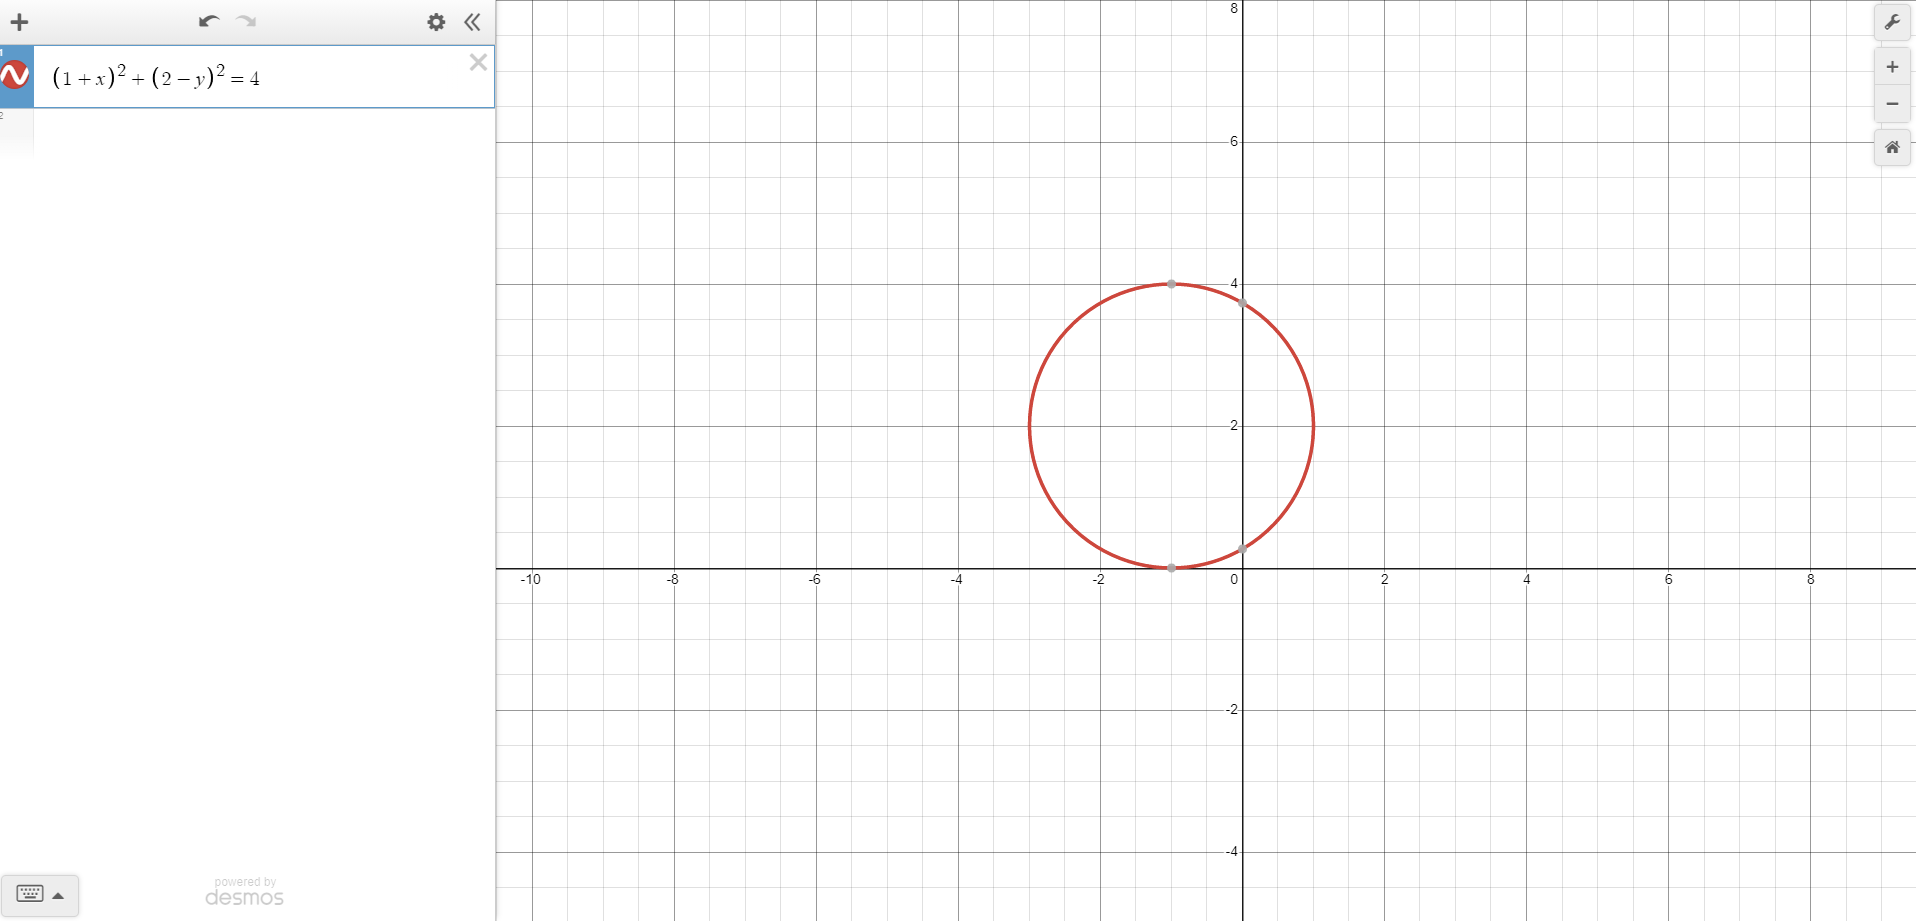
\includegraphics[scale = .3]{2a.png}
        
        \item For all the points greater than 4: \\ 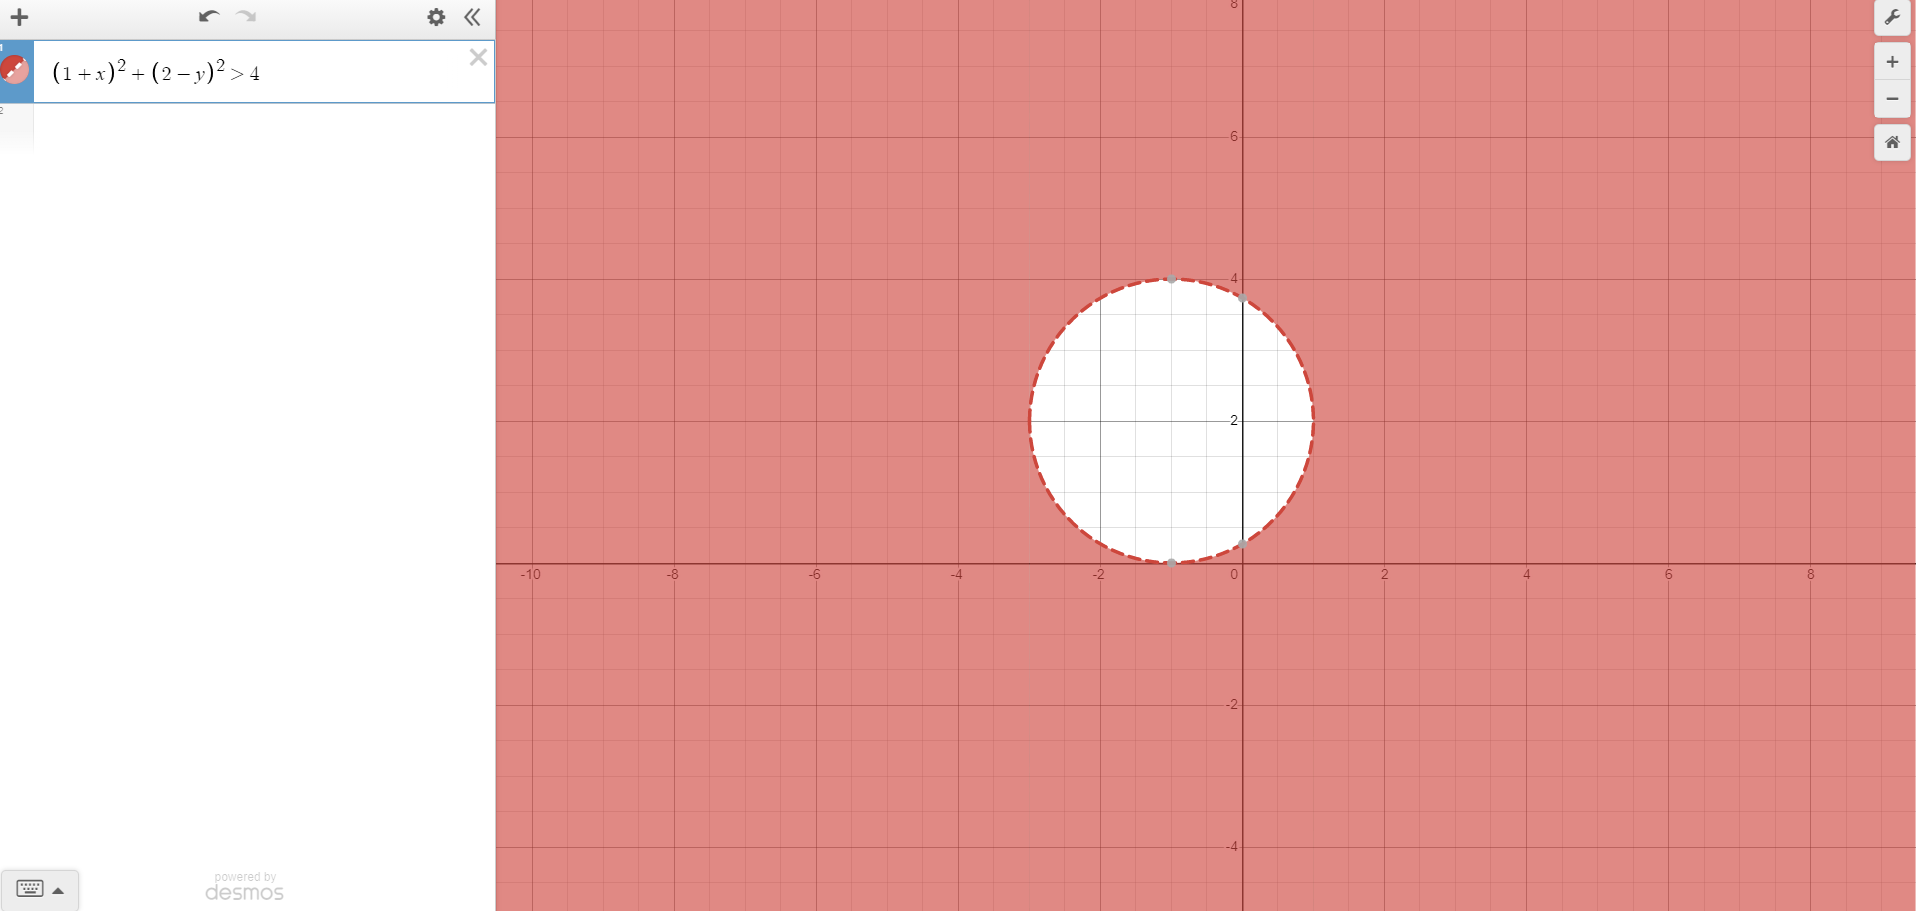
\includegraphics[scale = .3]{2b.png}\\
        For all the points less than or equal to 4: \\ 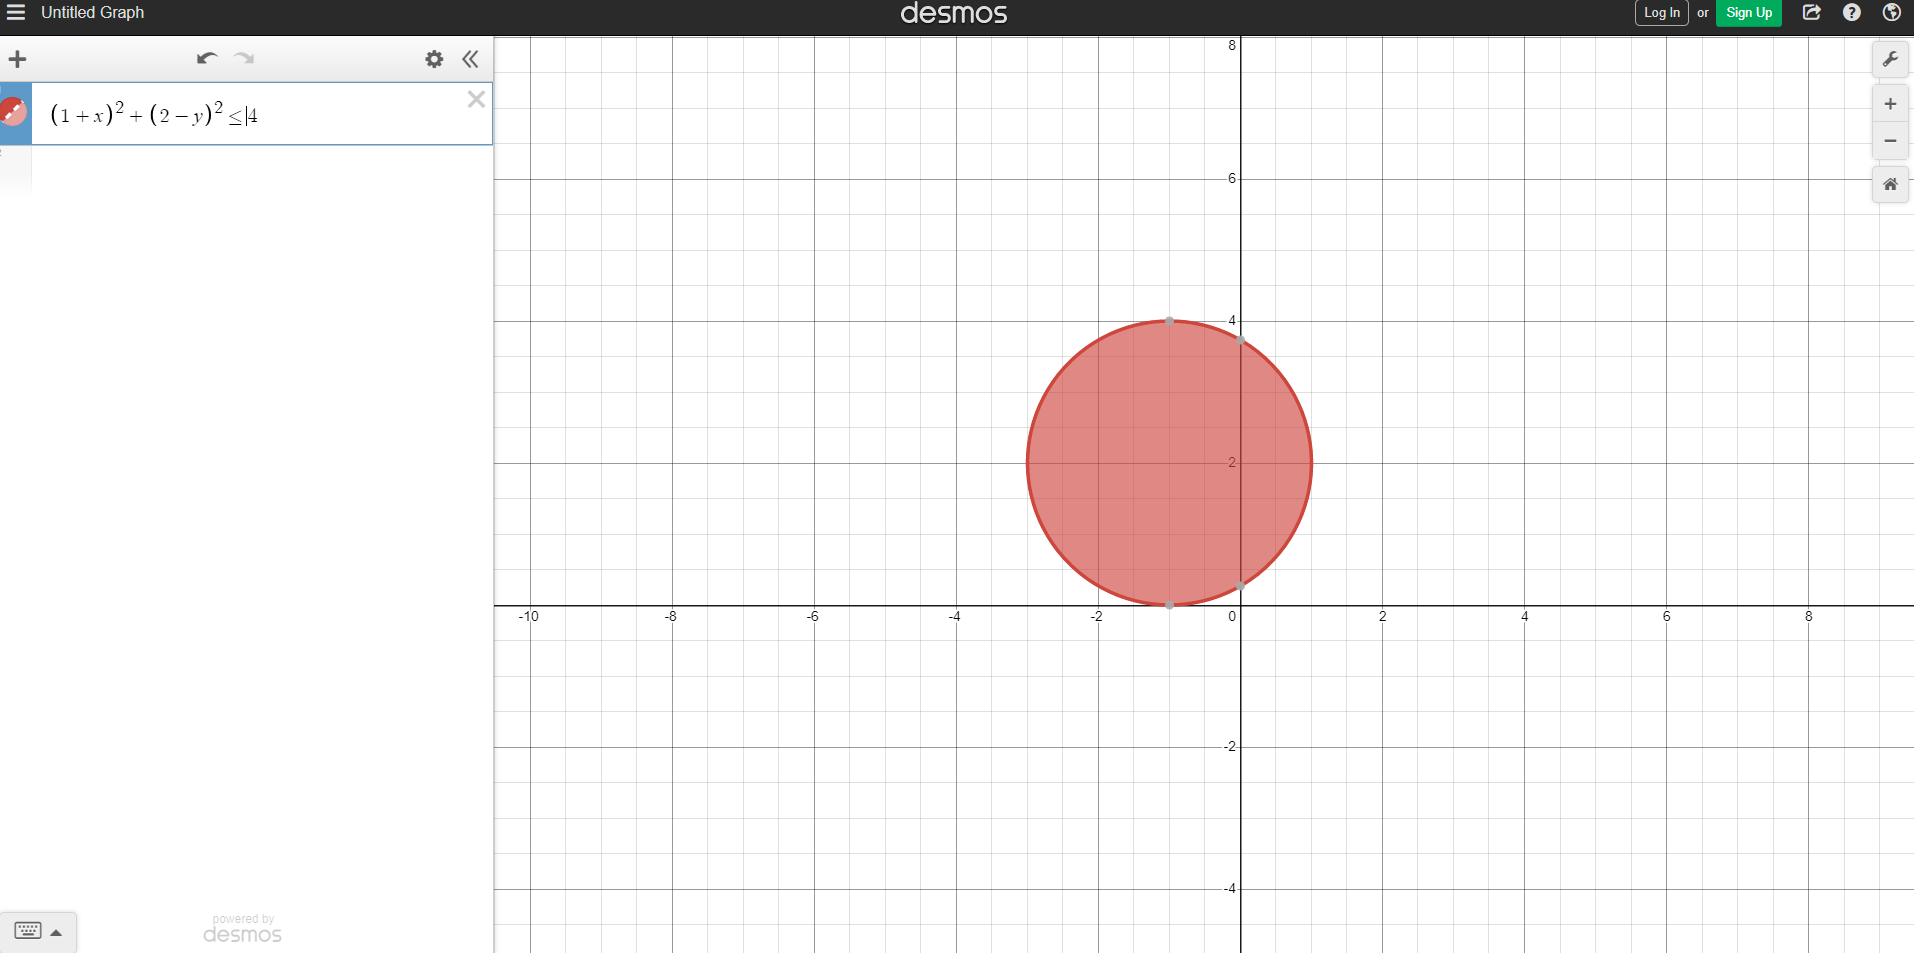
\includegraphics[scale = .3]{2b1.png}\\

        \item From the points plotted as well as the graph shaded where the points are 
        less than or equal to 4: \\ 
        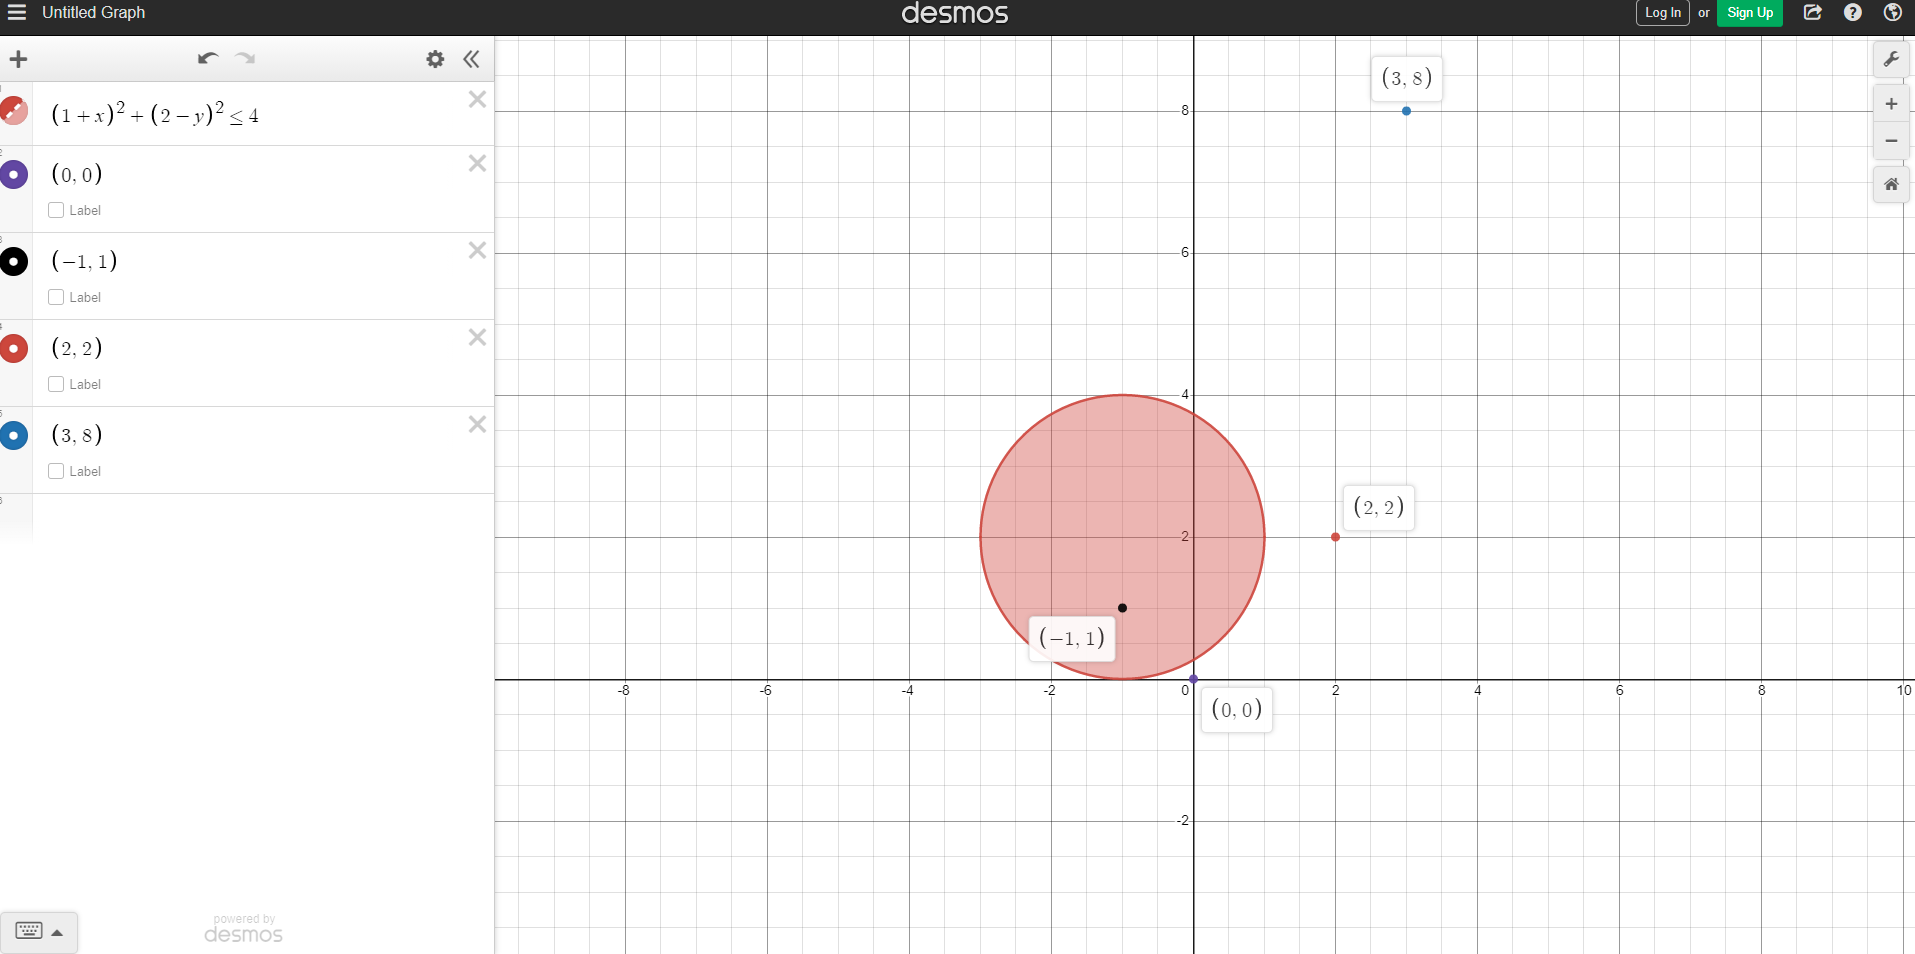
\includegraphics[scale = .3]{2c.png}\\
        We see only the point $(-1, 1)$ lies within the shaded region, and thus will 
        be the only one assigned to be red. All other points will be assigned to blue. 

        \item Looking at the equation of the circle, we find that the variable terms are 
        $X_1, X_1^2, X_2, X_2^2$. Thus, since the equation of a circle is a linear 
        combination of those four terms, the equation $(1-X_1)^2 + (2-X_2)^2 = 4$ is linear 
        in terms of $X_1, X_1^2, X_2, X_2^2$. 
    \end{enumerate}
\end{enumerate}

\end{document}